\documentclass[border=4pt]{standalone}
\usepackage{tikz}
\usetikzlibrary{arrows.meta,positioning,shapes.geometric}
\begin{document}
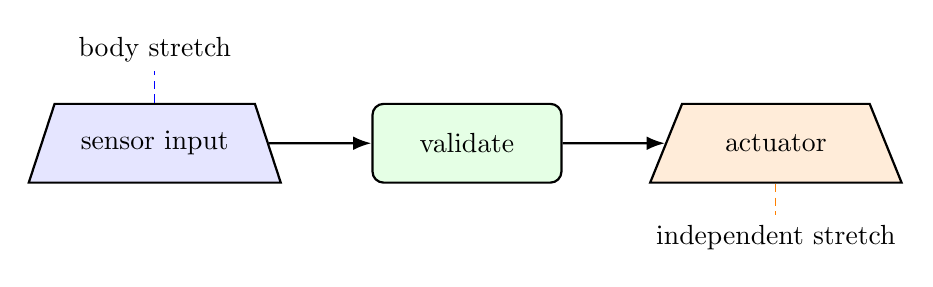
\begin{tikzpicture}[
  node distance=13mm,
  >=Latex,
  io/.style={
    trapezium,
    draw,
    thick,
    fill=blue!10,
    minimum width=32mm,
    minimum height=10mm,
    inner sep=2mm,
    trapezium angle=65,
    align=center
  }
]
  \node[io,trapezium stretches body] (input) {sensor input};
  \node[draw,thick,rounded corners,fill=green!10,right=of input,
    minimum width=24mm,minimum height=10mm] (filter) {validate};
  \node[io,trapezium stretches,right=of filter,fill=orange!15] (output) {actuator};

  \draw[-Latex,thick] (input.right side) -- (filter.west);
  \draw[-Latex,thick] (filter.east) -- (output.left side);
  \draw[densely dashed,blue] (input.top side) -- ++(0,4mm)
    node[above,black] {body stretch};
  \draw[densely dashed,orange] (output.bottom side) -- ++(0,-4mm)
    node[below,black] {independent stretch};
\end{tikzpicture}
\end{document}
